\subsection{Continuous Variable Resonance Combustor} \label{sec:5.res.4}

CVRC is a model rocket combustor designed and operated at Purdue University (Indiana, U.S.) to investigate combustion instabilities \cite{yu2008combustion}. This setup is called the Continuously Variable Resonance Combustor (CVRC) because the length of the oxidizer injector can be varied continuously, allowing for a detailed investigation of the coupling between acoustics and combustion in the chamber \cite{garby2013simulations}. The 2D/3D high-fidelity simulations of CVRC are expensive. Thus to get a fast analysis tool, a quasi-1D model has been proposed by Smith et al. \cite{smith2008computational} and further developed by Frezzotti et al. \cite{frezzotti2015determination,frezzotti2017numerical,frezzotti2018quasi}. 


The CVRC consists of three parts: oxidizer post, combustion chamber and exit nozzle, as shown in Fig. \ref{fig:radius}. The oxidizer is injected from the left end of the oxidizer post and meets the fuel that is injected through an annular ring around the oxidizer injector, at the back-step. The combustion happens in a region around the back-step. The combustion products flow through the chamber and exit the system from the nozzle.  Both the injector and the nozzle are operated at choked condition during the experiment. The length of the oxidizer post $L_{op}$ of the CVRC can be varied continuously, leading to different behavior of the combustion stability. In this paper, we will focus on the case with $L_{op}= 14.0$ cm, in which the combustion is unstable.

The geometry parameters of the quasi-1D CVRC with a oxidizer post length  $L_{op}= 14.0$ cm are shown in Table \ref{tab:geometry_parameters}.  The back-step and the converging part of the nozzle are sinusoidally contoured to avoid discontinuity of the radius that will invalidate the quasi-1D governing equations presented in the next subsection. 

\begin{figure}
	\centering
	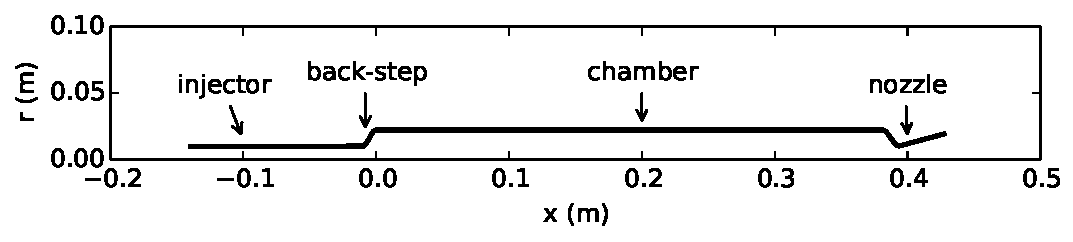
\includegraphics[width=0.8\linewidth]{pic/radius}
	\caption{Geometry of quasi-1D CVRC model.}
	\label{fig:radius}
\end{figure}

\begin{table} [h]
	\centering
	\caption{Geometry parameters of the quasi-1D CVRC with an oxidizer post length $L_{op}=14$ cm.}
	\centering
	\begin{tabular}{c c c c c c }
		\toprule
		\centering
		\multirow{2}{*}{Section} &
		\multicolumn{2}{c}{Oxidizer post} &
		\multirow{2}{*}{Chamber} &
		\multicolumn{2}{c}{Nozzle} \\
		\cmidrule(lr){2-3} \cmidrule(lr){5-6}
		& injector & back-step & & converging part & diverging part\\
		\midrule
		Length (cm) & 12.99 & 1.01 & 38.1 & 1.27 & 3.4 \\
		Radius (cm) & 1.02  & $1.02 \sim 2.25$ & 2.25 & $2.25 \sim 1.04$ & $1.04 \sim 1.95$ \\
		\bottomrule
		\label{tab:geometry_parameters}
	\end{tabular} 
\end{table}

The fuel is pure gaseous methane. The oxidizer is a mixture of 42\% oxygen and 58\% water (per unit mass). The oxidizer is injected in the oxidizer post at a temperature $T_{ox}=1030$ K so that both water and oxygen are in the gaseous phase. The operating conditions are listed in Table \ref{tab:operating-conditions}.

\begin{table} [h]
	\centering
	\caption{CVRC operating conditions.}
	\centering
	\begin{tabular}{l l l}
		\toprule
		\centering
		Parameter & Unit & Value \\
		\midrule
		Fuel mass flow rate, $\dot{m}_{f}$ & kg/s & 0.027   \\
		Fuel temperature, $T_{f}$ & K & 300   \\
		Oxidizer mass flow rate, $\dot{m}_{ox}$ & kg/s & 0.32   \\
		Oxidizer temperature, $T_{ox}$ & K & 1030   \\
		$O_2$ mass fraction in oxidizer, $Y_{O_2}$ & -- & 42.4\%   \\
		$H_2O$ mass fraction in oxidizer, $Y_{H_2O}$ & -- & 57.6\%   \\
		Mean chamber pressure & MPa & 1.34 \\
		Equivalence ratio, $E_r$ & -- & 0.8 \\
		\bottomrule
		\label{tab:operating-conditions}
	\end{tabular} 
\end{table}

For the combustion, we consider the one-step reaction model
\begin{equation*}\label{eq:combustion}
CH_4 + 2O_2 \rightarrow CO_2 + 2H_2O
\end{equation*}
We assume that the fuel reacts instantaneously to form products, allowing us to neglect intermediate species and finite reaction rates. As the equivalence ratio is less than one, there is oxidizer left after the combustion. Therefore, only two species need to be considered: oxidizer and combustion products.


The governing equations that describe the conservation of mass, momentum, and energy of the quasi-1D CVRC flow, are the quasi-1D unsteady Euler equations for multiple species, expressed in conservative form as
\begin{equation}\label{eq:5p2.1}
\frac{\partial }{\partial t} v + \frac{\partial }{\partial x} F_v = s_A + s_f + s_q.
\end{equation}
The conserved variable vector $v$ and the convective flux vector $F$ are
\begin{equation}\label{eq:5p2.2}
v= \left( \begin{gathered}
\rho A  \\
\rho uA  \\
\rho EA  \\
\rho Y_{ox} A \\
\end{gathered} \right), 
F = \left( \begin{gathered}
\rho uA  \\
\left(\rho u^2 + p\right)A  \\
\left(\rho E + p\right)uA  \\
\rho uY_{ox} A \\
\end{gathered} \right),
\end{equation}
where $\rho$ is the density, $u$ is the velocity, $p$ is the pressure, $E$ is the total energy, $Y_{ox}$ is the mass fraction of oxidizer, and $A=A(x)$ is the cross section area of the duct. The pressure $p$ can be computed using the conserved variables as
\begin{equation}\label{eq:total-engery}
E = \frac{p}{\rho (\gamma - 1)} + \frac{u^2}{2} - C_p T_{ref},
\end{equation}
where $T_{ref}$ is the reference temperature and is set as 298.15 K in this paper. The temperature $T$ is recovered from the equation of state $p = \rho R T$. The gas properties  $C_p$, $R$ and $\gamma$ are computed as $C_p= \sum C_{pi}Y_i$, $R=\sum R_iY_i$ and $ \gamma= C_p/(C_p-R)$, respectively. 

The source terms are
\begin{equation} \label{eq:5p2.3}
s_A = \left( \begin{gathered}
0  \\
p \frac{dA}{dx}  \\
0  \\
0 \\
\end{gathered} \right), 
s_f = \left( \begin{gathered}
{\dot \omega}_f  \\
{\dot \omega}_f u  \\
{\dot \omega}_f \left(h_{0}^{f} + \Delta h_{0}^{rel} \right)  \\
{\dot \omega}_{ox} \\
\end{gathered} \right), 
{s_q} = \left( \begin{gathered}
0  \\
0  \\
q'  \\
0 \\
\end{gathered} \right),
\end{equation}
where $\dot{\omega}_f$ is the depletion rate of the fuel, $\dot{\omega}_{ox}$ is the depletion rate of the oxidizer, $h_0^f$ is the total enthalpy of the fuel, $\Delta h_{0}^{rel}$ is the heat of reaction per unit mass of fuel and $q'$ is the unsteady heat release term. $s_A$ accounts for area variations, $s_f$ and $s_q$ are related to the combustion. $s_f$ represents the addition of the fuel and its combustion with the oxidizer, which in turn results in the creation of the combustion products. The depletion rate of the fuel is
\begin{equation}\label{eq:5p2.4}
\dot{\omega}_{f}= \frac{k_f \dot{m}_f Y_{ox} \left(1+sin\xi\right)}{l_f-l_s},
\end{equation} 
where
\begin{equation}\label{eq:5p2.5}
\xi= -\frac{\pi}{2} + 2\pi\frac{x-l_s}{l_f-l_s}, \hspace{0.5cm} \forall \hspace{0.2cm} l_s < x < l_f.
\end{equation}
The setting of the fuel injection restricts the combustion to the region $l_s < x < l_f$. The reaction constant $k_f$ is selected to insure that the fuel is consumed within the specified combustion zone. The depletion rate of the oxidizer is computed by 
\begin{equation}\label{eq:5p2.6}
\dot{\omega}_{ox} = C_{o/f} \dot{\omega}_f,
\end{equation}
where $C_{o/f}$ is the oxidizer-to-fuel ratio.

The unsteady heat release term $q'$, also called the combustion response function, models the coupling between acoustics and combustion. In this paper, we use the combustion response function designed by Frezzotti et al. \cite{frezzotti2017numerical,frezzotti2018quasi}, which is a function of the velocity, sampled at specific abscissa $\hat{x}$ that is almost coincident with the antinode of the first longitudinal modal shape, with a certain time lag $t_0$, i.e.,
\begin{equation}\label{eq:5p2.7}
q'\left( x,t\right) = \alpha g\left(x\right)  A\left(x\right) \left[ u\left( \hat{x},t-t_0 \right) - \bar{u}\left( \hat{x} \right) \right].
\end{equation}
Here $\bar{u}$ is the time averaged velocity, estimated with the steady-state quasi-1D model assuming $q'=0$, and $g(x)$ is a Gaussian distribution  
\begin{equation}\label{eq:5p2.8}
g\left(x\right)= \frac{e^{-\frac{\left(x-\mu\right)^2}{2\sigma^2}}}{\sqrt{2\pi\sigma^2}},
\end{equation}
where $\mu$ is the mean and $\sigma$ is the standard deviation. The amount of heat release due to velocity oscillations is controlled by the parameter $\alpha$.

The boundary conditions for the quasi-1D CVRC flow include the fixed mass flow rate and the stagnation temperature at the head-end of the oxidizer injector, and the supersonic outflow at the exit of the nozzle.

Prior to unsteady simulation, the quasi-1D CVRC needs to be excited, which can be achieved by adding a perturbation to the steady-state solution. The perturbation is added by forcing the mass flow rate with a multi-sine signal
\begin{equation}\label{eq:5p2.9}
\dot{m}_{ox} \left(t\right)= \dot{m}_{ox,0} \left[1 + \delta\sum_{k=1}^{K}  sin\left(2\pi k\Delta f t\right) \right],
\end{equation}
where $\dot{m}_{ox,0}$ is the oxidizer mass flow rate in Table \ref{tab:operating-conditions}, $\Delta f$ is the frequency resolution and $K$ is the number of frequencies. In this paper, $\Delta f = 50 $ Hz and $K=140$, resulting in a minimal frequency of 50 Hz and a maximal frequency of 7000 Hz. $\delta$ is required to be small to control the amplitude of the perturbation and is set as 0.1\%.

The procedure of the unsteady simulation of the quasi-1D CVRC flow includes three steps:
\begin{enumerate}
	\item  Compute the steady-state solution by setting $\dot{m}_{ox}=\dot{m}_{ox,0} $ and $q'=0$.
	\item  Excite the system by adding a perturbation to the oxidizer mass flow rate according to (\ref{eq:5p2.7}) and setting $q'=0$.
	\item  Perform the unsteady simulation by turning on the combustion response function $q'$ in (\ref{eq:5p2.3}) and turning off the oxidizer mass flow rate perturbation by setting $\dot{m}_{ox}=\dot{m}_{ox,0} $.	
\end{enumerate}

Note that the right hand side in \eqref{eq:5p2.3} suggests that, in general, mass, momentum, and energy is not conserved. Furthermore, the complex coupling of the variables in \eqref{eq:5p2.3} prohibits the application of complex and implicit time integration schemes. Therefore, a quasi-skew-symmetric form, introduced in \eqref{eq:3.7}, is considered for \eqref{eq:5p2.3}. This allows us to benefit from stability properties of skew-symmetric forms while using an explicit time integration scheme.

Introduction of an artificial viscosity is essential for a robust and long time-integration of \eqref{eq:5p2.3}. Common discretization schemes for \eqref{eq:5p2.3} are often dissipative, e.g. the Lax-Friedrich scheme used in \cite{Wang:255719}. Since the skew-symmetric discretization is non-dissipative, we modify \ref{eq:5p2.3} to write
\begin{equation} \label{eq:5p2.10} 
	\frac{\partial }{\partial t} v + \frac{\partial }{\partial x} F = s_A + s_f + s_q + d, \quad d = (0,\frac{\partial }{\partial x} \tau,0,0)^T,
\end{equation}
with $\tau = \mu \partial (u A)/ \partial x$, and $\mu = 6\times 10^{-5}$. This type of artificial viscosity is chosen due to its simplicity. This, however, can be replaced with a more moderate and sophisticated method. The three-stage Runge-Kutta (SSP RK3) \cite{jiang1996efficient} is used to then integrate \eqref{eq:5p2.10} in time.
The pressure profile for the steady state, with $q'=0$, and the pressure oscillatory mode in the unsteady phase is presented in \Cref{fig:5p2.2a}. We report that the added viscous term affects the level of pressure in the steady state and the aplitude of oscilations in the unsteady mode, compared to \cite{Wang:255719}.

\begin{figure}[t]
\centering
\begin{subfigure}[]{0.47\linewidth}
	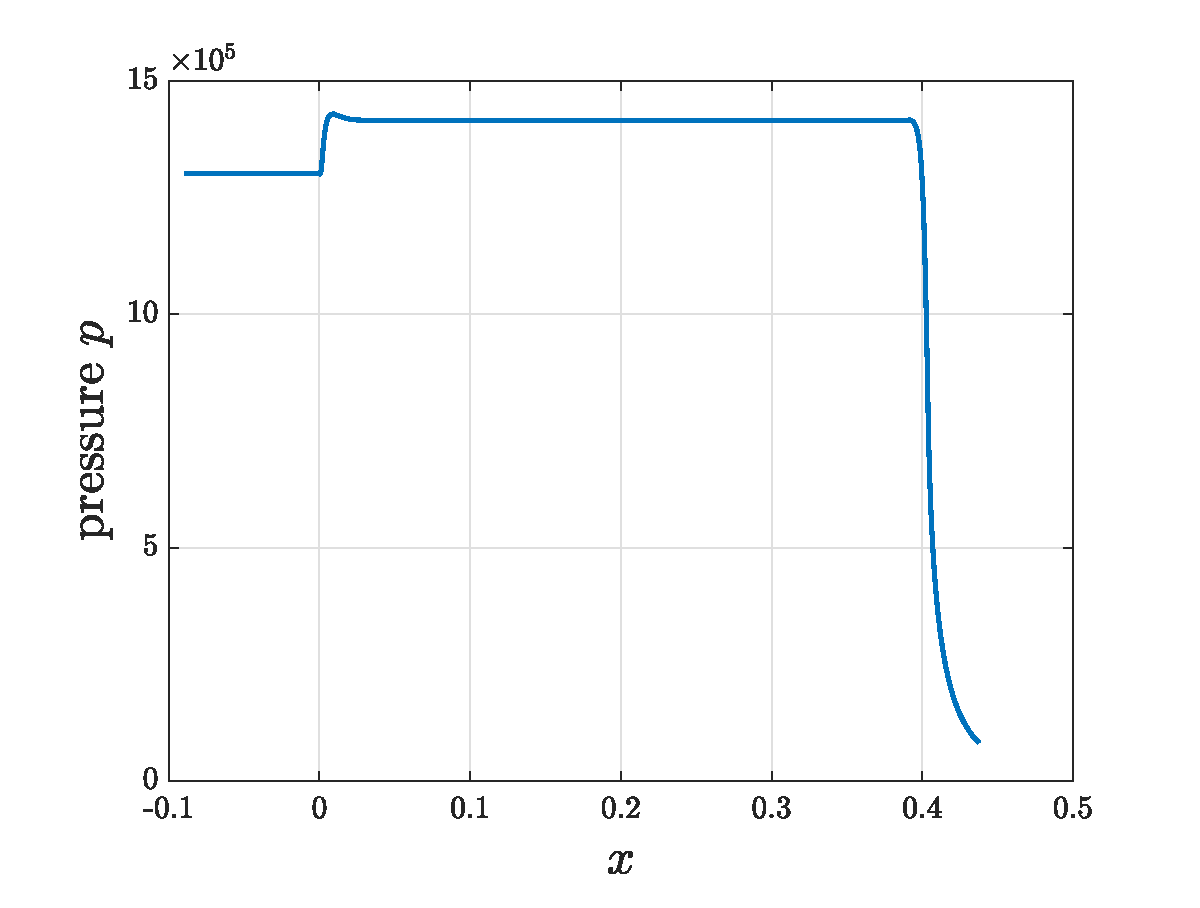
\includegraphics[width=\textwidth]{./pic/init_pressure}
	\caption{} \label{fig:5p2.2a}
\end{subfigure}
\begin{subfigure}[]{0.47\linewidth}
	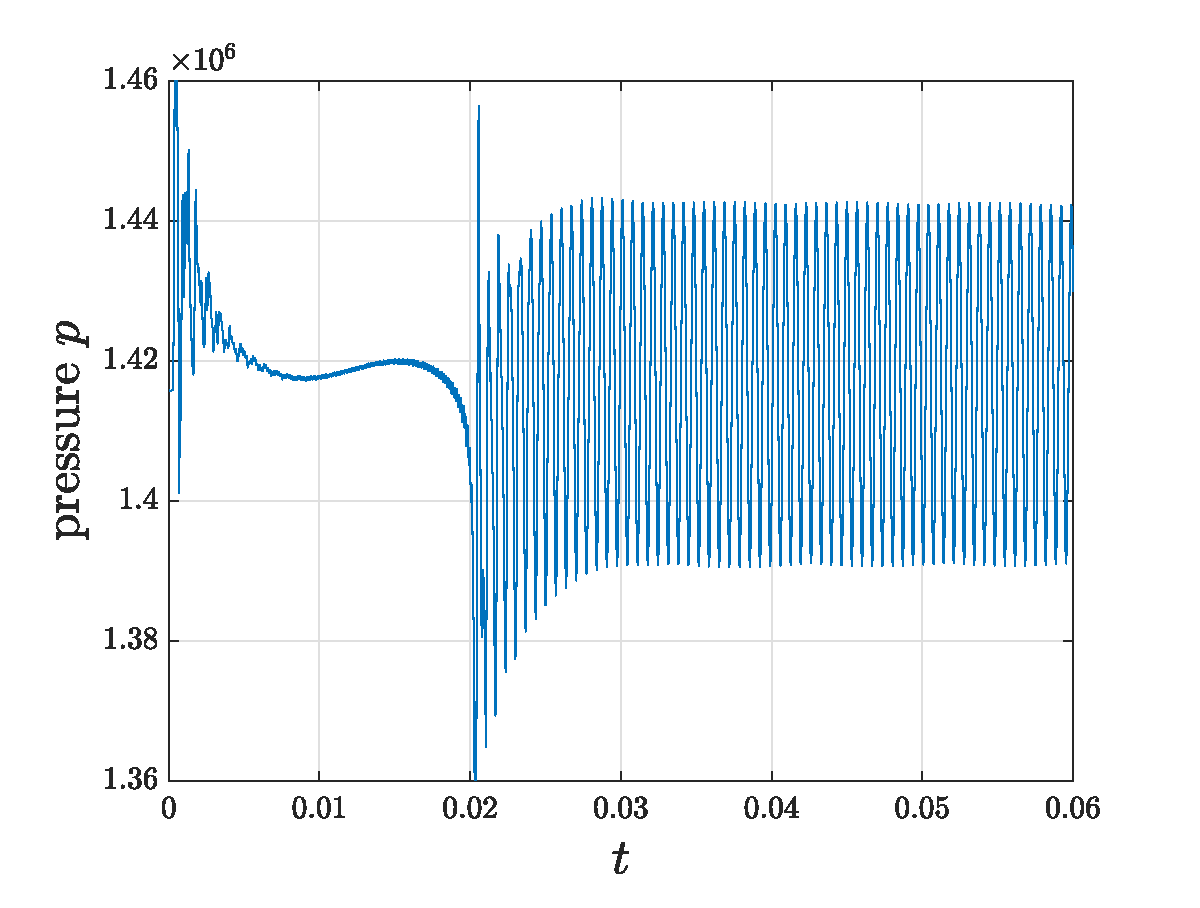
\includegraphics[width=\textwidth]{./pic/init_osc}
	\caption{} \label{fig:5p2.2b}
\end{subfigure} \\
\begin{subfigure}[]{0.47\linewidth}
	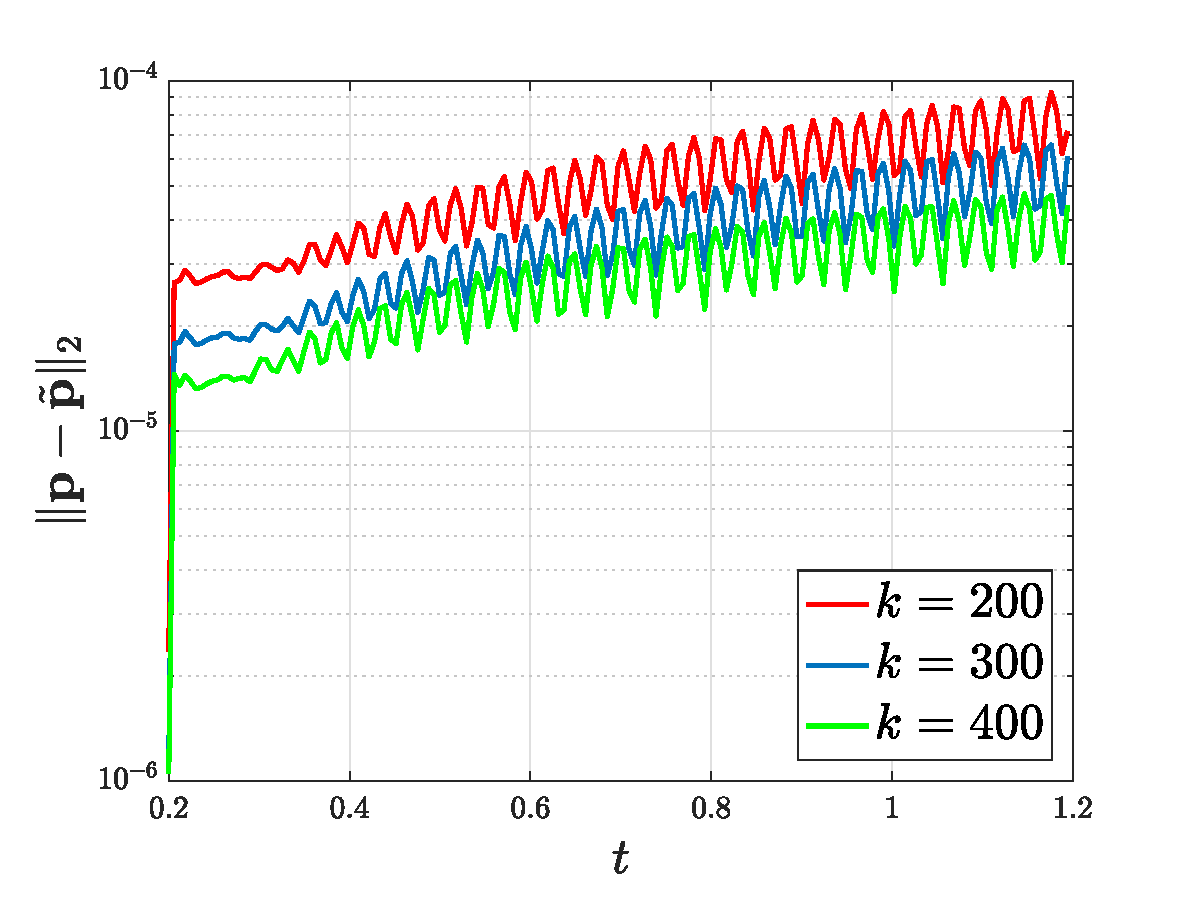
\includegraphics[width=\textwidth]{./pic/p_error}
	\caption{} \label{fig:5p2.2c}
\end{subfigure}
\begin{subfigure}[]{0.47\linewidth}
	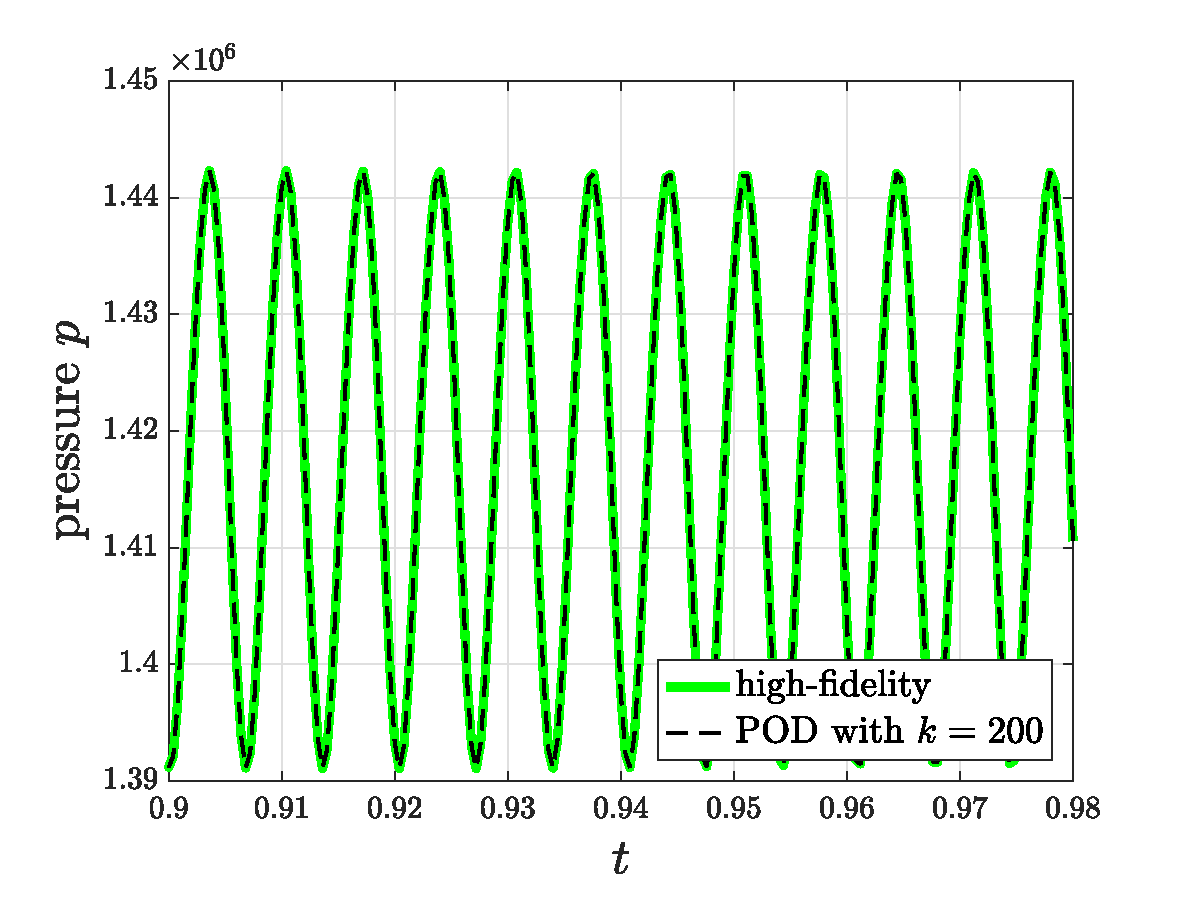
\includegraphics[width=\textwidth]{./pic/rom_freq}
	\caption{} \label{fig:5p2.2d}
\end{subfigure}
\caption{(a) Pressure profile of the steady state. (b) Oscillatory mode of pressure located at $x=0.36$ for the unsteady flow. (c) Relative error between the high-fidelity and approximated pressure. (d) Approximation of the oscillations. }
\label{fig:5p2.2}
\end{figure}

The discontinuities that appear in the solution of \eqref{eq:5p2.10} suggests that a, relatively, large basis is required to resolve fine strucutres in the solution. In this paper, a POD basis is generated with $k=200$, $k=300$ and $k=400$ number of basis vectors. To avoid basis changes in reduced system, only one POD basis is considered for $\rho$, $\rho u$ $\rho E$ and $\rho Y_{ox}$. The explicit SSP RK3 is then used to integrated the reduced system in time, for the unsteady system. The source terms are evaluated in the high-fidelity space and then projected onto the reduced space. However, in principle, the DEIM can be applied to accelerate this evaluation. 

\Cref{fig:5p2.2c} shows the approximation error of the pressure, due to MOR. It is observed that the approximation is coherently enhanced as the number of basis vectors are increase. Furthermore, the approximated solution maintains high accuracy over a relatively long time-integration. The oscilations of pressure is demostrated in \Cref{fig:5p2.2d}. It is seen that the overall behaviour of pressure is well approximated using the reduced system. Similar results are obtained for a POD basis with higher number of modes.

We note that the discrete form of \eqref{eq:5p2.10} is not in the full skew-symmetric form. Nontheless, the quisi-skew-symmetric discretization provides a remarkable stability preservation.
